\section{Decorator}

O padrão Decorator permite adicionar responsabilidades a um 
objeto de forma dinâmica. Essa dinamicidade é alcançada 
substituindo a herança por uma agregação, permitindo que a 
classe decorada delegue responsabilidades para as classes que 
a estendem. As classes de extensão implementam uma 
interface em comum com as classes decoradas, também 
armazenando em seus atributos um objeto que também 
implementa essa interface. Dessa forma, uma classe 
de extensão pode tanto referenciar outra classe de extensão 
quanto o objeto decorado, formando uma estrutura de pilha 
onde o elemento ao fundo é o objeto decorado. Ele será o 
alvo das operações acumuladas de todos os extensores 
presentes na estrutura. O diagrama de classes que 
demonstra essa estrutura pode ser visto na figura 
\ref{decorator_struct}.

O maior problema resolvido pelo Decorator é a grande 
quantidade de classes que deveriam existir caso houvessem 
muitas extensões para uma classe. O problema cresce ainda 
mais quando é necessário que essas funcionalidades mudem 
dinamicamente, gerando diversas combinações de grupos de 
funcionalidades possíveis.

\begin{figure}[htb]
	\caption{\label{decorator_struct}Estrutura do Decorator}
	\begin{center}
	    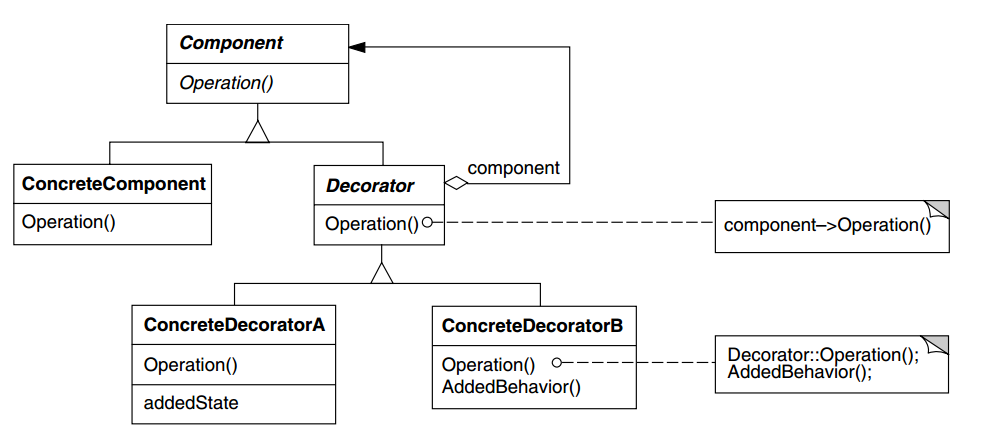
\includegraphics[scale=0.4]{5_padroes-contexto-funcional/5.2_estruturais/5.2.4_decorator/diagram.png}
	\end{center}
\end{figure}

\subsection*{Exemplo Orientado a Objetos}

Como exemplo, é apresentado uma ferramenta  
gráfica que permite que diversas funcionalidades, 
como bordas ou barras de rolagem, possam ser adicionadas 
a qualquer componente. Ao invés de usar herança, 
o que exigiria que houvesse uma subclasse para cada 
combinação de funcionalidades e elementos gráficos, 
o padrão Decorator é utilizado. Por exemplo, um 
elemento de texto pode ser decorado com uma barra 
de rolagem ou com uma borda. A figura \ref{decorator_exemplo} 
demonstra o diagrama de classes para esse caso, 
onde uma classe TextView implementa uma interface 
VisualComponent, assim como a classe abstrata Decorator, 
que armazena em seus atributos um objeto do tipo 
VisualComponent. As classes ScrollDecorator e 
BorderDecorator herdam de Decorator, o que faz com que 
elas implementem VisualComponent. Uma das 
possibilidades desse cenário é que um objeto do tipo 
ScrollDecorator armazene um BorderDecorator, que 
por sua vez armazenará um TextView. A operação 
Draw será chamada, em sequência, para cada 
elemento da pilha, resultando no TextView 
com as funcionalidades desejadas. O código 
\ref{oodecorator} traz a implementação dessa 
abordagem.

\begin{figure}[htb]
	\caption{\label{decorator_exemplo}Exemplo de Decorator}
	\begin{center}
	    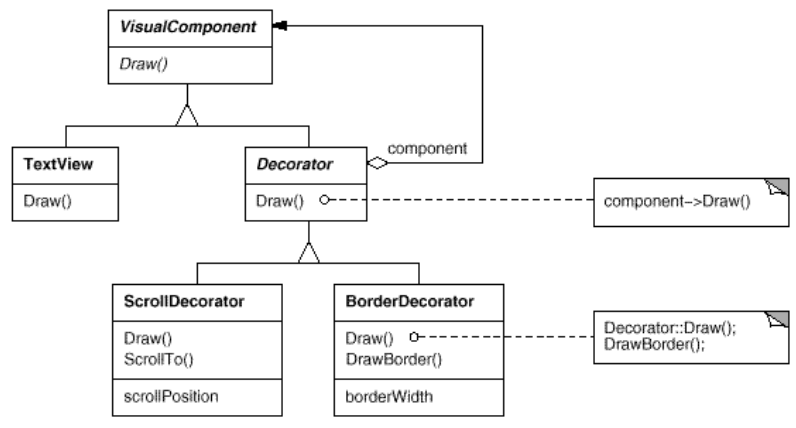
\includegraphics[scale=0.4]{5_padroes-contexto-funcional/5.2_estruturais/5.2.4_decorator/decorator_exemplo.png}
	\end{center}
\end{figure}

\begin{lstlisting}[caption={Decorator Orientado a Objetos},label=oodecorator]

trait VisualComponent{
	def Draw();
}

class TextView() extends VisualComponent {
	def Draw() {
		// Desenha o TextView
	}
}

abstract class Decorator(val component : VisualComponent){
	def Draw() {
		component.Draw();
	}
}

class ScrollDecorator() {
	
	var scrollPosition : Int;

	def Draw() {
		// Desenha o Scroll
		super.Draw();
	}
}

class BorderDecorator() {
	
	var borderWidth : Int;

	def Draw() {
		// Desenha o Border
		super.Draw();
	}
}

\end{lstlisting}

\subsection*{Contexto Funcional}

O mesmo objetivo é alcançado de forma simples através de 
composição de funções. Caso um valor precise ser decorado 
com diversas funções, uma função recebe esse valor como 
parâmetro e uma lista com todas as funcionalidades que irão 
estendê-lo. Essas funções são então chamadas uma por uma, 
gerando também uma pilha de chamadas que finalmente 
retorna o resultado da combinação de todas as operações.

\begin{lstlisting}[caption={Decorator Funcional},label=fpdecorator]
    

    
\end{lstlisting}